\section{Erstes Praktikum}

\subsection{Wahl unserer Ware}
Wir haben uns darauf geeinigt Spaceships, sprich Raumschiffe zu vertreiben. Diese werden aus seperat Lieferbaren Produkten wie beispiels weise Laserkanonen oder Warpantriebseinheiten zusammengesetzt. 

\subsection{Architektur\"ubersicht}
Wir brauchen als Komponenten eine Warenverwaltung, eine Kundenverwaltung, eine Rechnungsverwaltung und eine Businesslogic mit einer Web-GUI.

\begin{figure}[h]
  \caption{\"Ubersicht}
  \label{fig:archi}
  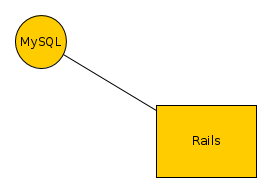
\includegraphics[scale=1.0]{architektur}
\end{figure}

\subsection{Sequenzdiagramm f\"ur eine Warensuche}
\begin{figure}[h]
  \label{fig:suche-seq}
  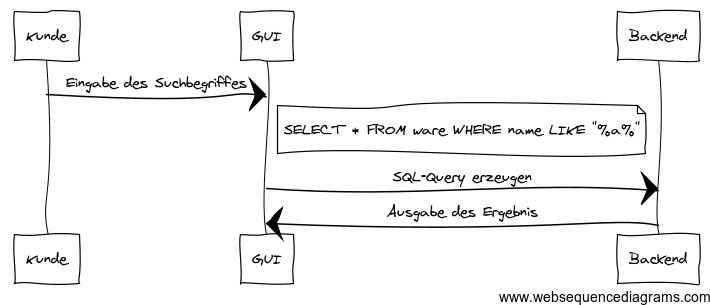
\includegraphics[scale=0.5]{suche-sequenz}
\end{figure}


\subsection{Begr\"undung der gew\"ahlten Tenchnologien}
Zur Debate stand, welche Programmiersprache bzw. welche Scriptsprache, welchen Webserver und welches Datenbankmanagementsystem wir f\"ur die Entwicklung des Webshops verwenden. Zur Option stellten wir uns hier aufgrund der Bekanntheit Ruby on Rails und PHP.

\begin{figure}[h]
	\caption{Vergleich zwischen Rails und PHP}
	\cite{tbray}
	\label{fig:vergleich}
	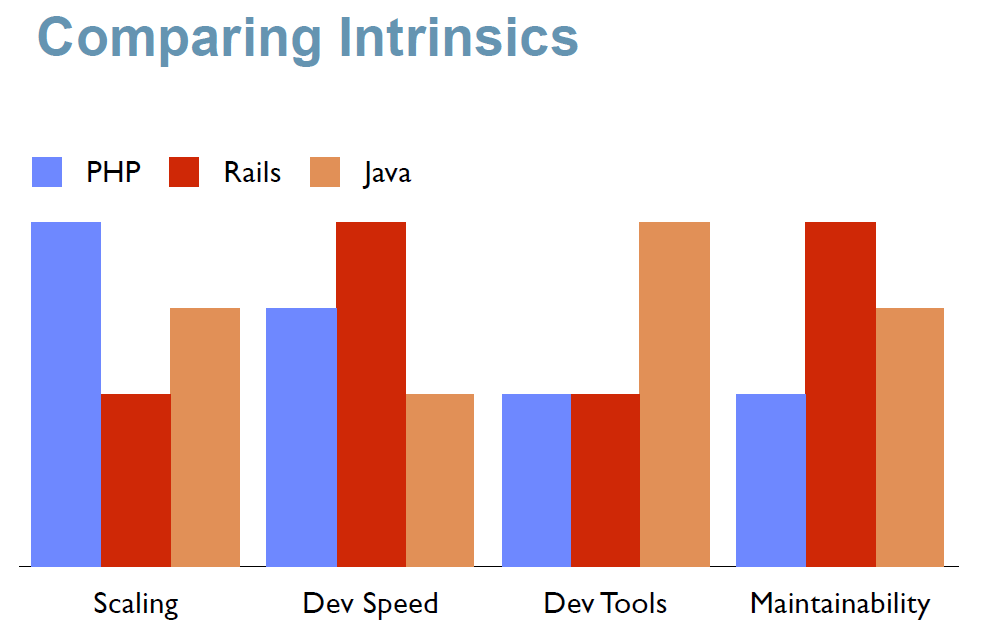
\includegraphics[scale=0.4]{complang}
\end{figure}

In Abbildung \ref{fig:vergleich} zu sehen, ist ein Vergleich zwischen Java, Ruby on Rails und PHP. Wir werden aufgrund der Entwicklungsgeschwindigkeit, der Wartbarkeit und dem Grund, dass wir Ruby in Programmieren I verwendeten, Ruby on Rails verwenden. Offen bleibt nun, welches Datenbankmanagementsystem und welchen Webserver wir verwenden. Da Rails nativ einen Webserver bereitstellt, werden wir diesen verwenden. Die Anbindung an ein DMBS gestaltet Rails auch problemlos. Wir stellten uns SQLite und MySQL zur Option. Nach einigen Artikeln, welche diese Vergleichen f\"allt auf, dass MySQL eher f\"ur gro{\ss}e Anwendungen geignet sind, welche auf Skalierbarkeit und Performanz Wert legen. SQLite hingegen soll sehr gut f\"ur Prototypen von Datenbanken, eine schnelle Entwicklung geeignet sein. Hierbei legt SQLite keinen Wert auf Nutzerverwaltung und Skalierbarkeit. Nachteile von MySQL ist, dass es eine h\"ohere Komplexit\"at in der Einrichtung aufweist. Beide verwenden offensichtlicher weise SQL. Letztendlich haben wir uns f\"ur MySQL entschieden, da wir den Umgang mit einem schwergewichtigen DBMS \"ueben m\"ochten. In Ruby on Rails werden wir Gems verwenden, welche kleine Erweiterungen f\"ur das System sind. Die verwendeten Gems sind \texttt{paperclip} und \texttt{mysql}.

\subsection{Design der Datenbank}
\label{sec:dbdesign}
Wir wurden gebeten eine Ware zu vertreiben, welche aus anderen Waren zusammengesetzt werden kann. Dieses Modell wird dadurch eine Rekursion enthalten, da wir die Bauteile der Produkte eventuell ebenfalls vertreiben w\"urden. Interessant ist also die Ware mit ihrem Namen, einer Beschreibung, einem Bild der Ware und ihrer Zusammensetzung. Hierf\"ur verwenden wir eine rekursive Relation von der Ware auf die Ware selbst.  

\begin{wrapfigure}{R}{0.5\textwidth}
  	\begin{center}
    	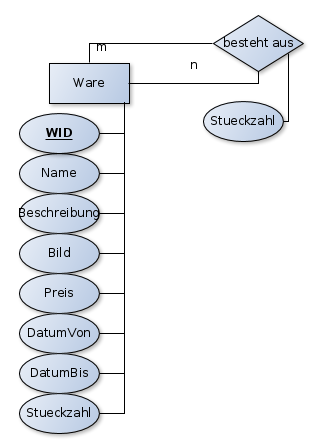
\includegraphics[scale=0.6]{databaseWare}
 	 \end{center}
   \caption{ERM der Ware und ihrer Struktur}
\end{wrapfigure}

\subsection{Dokumentation}

\subsubsection{Installation der Software Komponenten unter Arch Linux}
Das Installieren der Softwarekomponenten hat sich unter Linux als \"au{\ss}erst einfach erwiesen. Unter der Distribution Arch Linux musste man zun\"achst MySQL, nodejs, ruby und die Gems von Ruby installieren. Die ersten drei waren mit dem Befehl \texttt{sudo pacman -S mysql nodejs ruby} abgehandelt. F\"ur MySQL mussten wir  zus\"atzlich \texttt{mysql\_secure} \texttt{\_installation} eingeben um das Passwort von root zu \"andern. Nun muss man noch den Daemon mit \texttt{sudo systemctl} \texttt{start mysqld} starten. Wenn man m\"ochte, dass der Daemon beim n\"achsten hochfahren des Rechners automatisch startet, gibt man zus\"atzlich \texttt{sudo systemctl enable mysqld} ein. F\"ur die abschlie{\ss}ende Installation der gems nutzten wir \texttt{gem install mysql rails paperclip}. 

\subsubsection{Umsetzung der Datenbank}
Um eine Erzeugung einer Datenbank wird sich in nur indirekt gek\"ummert, da Rails die Anbindung an Rails vollst\"andig \"ubernimmt. Ebenfalls arbeitet Rails intern mit Relationen, weshalb keine Fremdschl\"ussel in der Datenbank auftauchen. Desweiteren gestattet uns Rails durch \texttt{belongs\_to} und \texttt{has\_many} in den Modellen diese Relationen zu gestallten. Bilder werden in unserer Datenbank mittels Name, Typ, Gr\"o{\ss}e und dem letzten Update gespeichert. F\"ur die Verwaltung dieser haben wir uns f\"ur das gem Paperclip entschieden. 

\subsubsection{Nutzeroberfl\"ache}
Die Nutzeroberfl\"ache haben wir uns durch Rails generieren lassen. Eine Validierung der Daten bei der Warenerzeugung findet in den Modellen statt. Wenn diese fehlschl\"agt, wird der Nutzer aufgefordert seine Eingabe zu korrigeren. Die Validierung \"uberpr\"uft lediglich ob die Daten f\"ur das Anlegen neuer Waren vorhanden sind.  
